\lhead{\emph{\leftmark}}  
\chapter{Evaluation}
\label{chap:evaluation}
% how far can we umplify a new system
In order to ensure that the results presented in this thesis are of high engineering quality and are as valid as possible from a scientific perspective, several approaches need to be followed. We validated our reverse engineering approach  by studying the application of our approach on various software systems. We adopted a \textbf{four-phase validation process} with the following steps:

\begin{description}

\item[Testing Phase]
Unit testing is carried out following a Test Driven Development approach (TDD).

\item[Pre-validation Phase]
Small Java systems written in high quality Java code, with known corresponding models, are employed to validate the accuracy of the transformations performed by the Umplificator.

\item[Initial Phase]
Medium and large  open-source projects are employed to validate the accuracy of the transformations and mapping rules. This set of open source projects will be known as the \textbf{`training set'}. The goal of this phase is to ensure the correctness and precision of the transformations on the training set.

\item[Machine Learning-Based Phase]
In this phase, we umplify a set of randomly selected systems, the \textbf{`testing set'} and assess the extent to which our transformations still work. We document the errors encountered during this phase of validation.

\end{description}

In general all four of the above phases are conducted in an iterative manner. In other words, we develop the Umplificator in small chunks that are validated at the same time.

This chapter is organized as follows: in the next sections we present each of the four phases of validation including the results obtained.  Finally, we provide extended details on the largest systems that were umplified during the four phases. 

\section{Testing Phase}
\label{sec:testingUmplificator}
As illustrated in Section \ref{chap:tool}, the Umplificator includes: a \textbf{parser}, a \textbf{model extractor}, a \textbf{transformer} and an Umple code \textbf{generator}. Each of the components is independently tested to ensure high quality as illustrated in Figure \ref{fig:testingPhase}. The testing phase explained in this section concerns only the testing process within the scope of the Umplificator.  In other words, we are testing the Umplificator implementation and \textbf{not} testing the set of possible umplified systems generated using our tool. 

%In fact, we only test that the outputs (Umple code) are syntactically correct. To achieve the additional level of %testing to validate the semantics of systems generated by the Umplificator, one must run or build a test suite against %those generated systems.

% The above is confusing when read in conjunction with the next sentence. Are you saying you do do have a test suite against a a generated system or not. I think the idea is that this is in a later stage. Rephrase to clarify.
% MG. Yes, I was actually contradicting myself, I wrote this before. I removed most of the paragraph.
% MG. Fixed.

At present there are over 135 tests that spans all components of the tool (parser, extractor, transformer, generator) and are run as part of our automated building process.

% MG. The above counts the semantic tests, but then how many syntactic tests are there.
% MG. 135 is actually my total number of tests.
In the subsequent sections we provide an overview of each aspect of the Umplificator's testing approach. 

\begin{figure}[h]
\centering
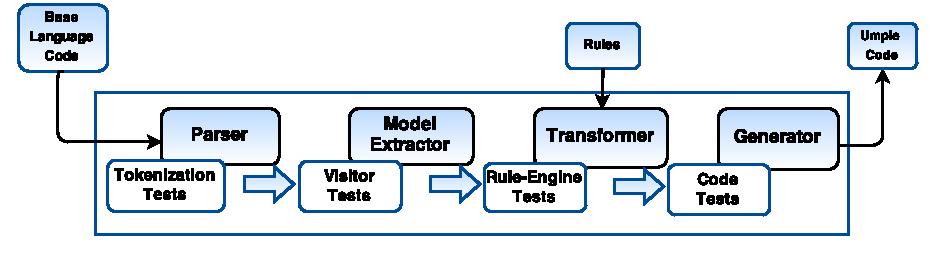
\includegraphics[width=1\textwidth]{Figures/testingPhase.pdf} 
\caption{Umplificator Testing Infrastructure}
\label{fig:testingPhase}
\end{figure}

\subsection{Testing the Base Language Code Parsers}

Testing the Umplificator parser is centered on the creation of the Abstract Syntax Tree (AST) from base language code. Our tests ensure that Base Language code is parsed and tokenized as we expect.

% Why do you call it AST DOM. AST would be more correct. DOM usually refers to the model of a web page.
% MG. This is how they called them, but I agree it is confusing. I removed it.
A simple parser test that verifies that the list of detailed problem reports (warnings, or compilation errors) noted by the compiler during the parsing or the type checking of the compilation unit (file) is what we expect, is shown in Listing \ref{lst:simpleFileWithTwoErrors}.
In this particular parser test, we are expecting two problems (compilation errors) since the input compilation unit contains two errors at two different locations in the code. The input code has been omitted. 

\begin{lstlisting}[style=java, label={lst:simpleFileWithTwoErrors}, caption=A Parser Test]
@Test
public void simpleFileWithTwoErrors()
{
  File testFile = new File(pathToInput+"SimpleFileWithTwoErrors.java");
  String code = SampleFileWriter.readContent(testFile);
  JavaParser javaParser = new JavaParser(); // JDT Parser
  CompilationUnit unit  = javaParser.parseUnit(code);
  Assert.assertEquals(2,unit.getProblems().length());
}
\end{lstlisting}

The pattern for parser-related test is presented in Listing \ref{lst:parserTestX}:

\begin{lstlisting}[style=java, label={lst:parserTestX}, caption=A pattern for parser tests]
@Test
public void parserTestX()
{
  // Step 1: Load external source file (Java or C++ file)
  // Step 2: Parse file (ensure parsing successful) 
  // Step 3: Verify tokenization
  // Step 4: Clean up
}
\end{lstlisting}

\subsection{Testing the Model Extractor}

Testing the model extractor ensures that from the tokens obtained through the parser we obtain a valid base language model representation (e.g. Java model, Umple model, CPP model). In particular, as we have implemented a visitor (software design pattern \cite{gamma1994design}) to traverse the different elements of the retrieved base language model, our tests certify that the visitor returns the desired number of elements.

% Ref to visitor pattern
% MG. Fixed. Gamma book for patterns
For instance, if the test input file contains (Listing \ref{lst:inputVisitor}): 

\begin{lstlisting}[style=java, label={lst:inputVisitor}, caption=Java input file for test]
package cruise.umplificator.visitorTestFiles;

 import java.util.*;
 import java.io.*;

 @SuppressWarnings("unused")
 public class InputForVisitorTest { 

  boolean result = true;
  char capitalC = 'C';
  byte b = 100;
  short s = 10000;
  int i = 100000;
  double d1 = 123.4;
  long creditCardNumber = 1234_5678_9012_3456L;

  InputForVisitorTest () { }

  InputForVisitorTest(byte b) {
   this.b=b;
  }

  public int getB(){
   return b;
  }
}
\end{lstlisting}

in the unit test shown in Listing \ref{lst:JavaVisitorTest} we assert that the (Java) visitor returns: 7 field declarations (Lines 17-20), 2 import declarations (Lines 23-27), 3 method declarations (Lines 37-41) and a package name `cruise.umplificator.visitorTestFiles' (Line 30-34).

% The following should have a listing number. Search the thesis for other listings without listing numbers
% MG.Fixed
% MG. Quote style is being fixed as well. `someting'

\begin{lstlisting}[style=java,label={lst:JavaVisitorTest}, caption=A JavaVisitorTest.java]
public class JavaVisitorTest {

String pathToInput;
JavaClassVisitor visitor ;
	
 @Before
 public void setUp() throws Exception {
  pathToInput = SampleFileWriter.rationalize("test/cruise/umplificator/visitorTestFiles/");
  File testFile = new File(pathToInput+"InputForVisitorTest.java");
  String code = SampleFileWriter.readContent(testFile);
  JavaParser javaParser = new JavaParser();
  CompilationUnit unit  = javaParser.parseUnit(code);
  visitor = javaParser.getJavaVisitor();
 }
	
 @Test
 public void field_declarations_returned_in_java_file()
 {
  Assert.assertEquals(7, visitor.numberOfFieldDeclarations());
 }
		
 @Test
 public void imports_returned()
 {
  int nbImports = visitor.numberOfImportDeclarations();
  Assert.assertEquals(2, nbImports);
 }
	
 @Test
 public void packages_returned()
 {
  String packageName = visitor.getPackageDeclaration().getName().getFullyQualifiedName();
  Assert.assertEquals("cruise.umplificator.visitorTestFiles", packageName);
 }

 @Test
 public void methods_returned()
 {
  int nbMethods = visitor.numberOfMethodDeclarations();
  Assert.assertEquals(3, nbMethods);
 }
\end{lstlisting}

\subsection{Testing the Transformer}

Testing the \textbf{transformer} involves ensuring that our Rule-Engine receives the input, fires the corresponding mapping rules and produces the expected output.
For instance, if the input of our tests below is the Java class presented in Listing \ref{lst:inputVisitor}, we expect all the assertions in the test class \textit{RulesAttributesTypesTest} to pass. The JUnit test class, as shown in Listing \ref{lst:testClassSetup}, contains a  method \textit{setUp()} that specifies the work to be done before running each test such as initializing instance variables. 

In Line 18 we parse the input file and create an Umple class that is inserted into the working memory of the Rule Engine. In Line 22, an Umple class is inserted into the Working memory (of Drools Rule Engine). Note that in Line 21  the desired \textbf{level of refactoring} includes Umple attributes (and excludes Umple associations) since the goal of this test class is to ensure the correct mapping between variables possessing certain characteristics and Umple attributes. Finally, we clean the working memory of the rule engine (Line 28).

\begin{lstlisting}[style=java, label=lst:testClassSetup, caption=RulesAttributesTypesTest class]
public class RulesAttributesTypesTest {

 String pathToInput;
 JavaClassVisitor visitor ;
 RuleRunner runner  = new RuleRunner();
 RuleService ruleService= new RuleService(runner);
 KieSession kieSession;
 UmpleClass uClass;
 CompilationUnit compilationUnit;
	
@Before
public void setUp() throws Exception {
 pathToInput = SampleFileWriter.rationalize("test/cruise/umplificator/visitorTestFiles/   InputForVisitorTest.java");
 File testFile = new File(pathToInput);
 String code = SampleFileWriter.readContent(testFile);
 visitor = new JavaClassVisitor();
 JavaParser javaParser = new JavaParser();
 javaParser.parseUnit(code);
 visitor = javaParser.getJavaVisitor();
 uClass = new UmpleClass("Test");
 kieSession = ruleService.startRuleEngine(RefactoringLevel.ATTRIBUTES);
 kieSession.insert(uClass);
}
 // test cases ...
 
 @After
 public void tearDown() throws Exception {
  runner.dispose();		
 }
}
\end{lstlisting}
% Fix Line X and Line Y in above to have correct line numbers
% MG. Done.

The unit test \textit{testNumberOfObjectsInWorkingMemory} in Listing \ref{lst:testNumberOfObjectsInWorkingMemory} ensures that at this point of time, there is only one element in the working memory (the Umple class inserted  before) since the mapping rules have not been fired yet.

\begin{lstlisting}[style=java, label=lst:testNumberOfObjectsInWorkingMemory, caption=Test asserting the working memory contents]
 @Test
 public void testNumberOfObjectsInWorkingMemory() {
   Assert.assertEquals(1, kieSession.getObjects().size());
 }
\end{lstlisting}

The unit test \textit{testCorrectMappingBetweenPrimitiveField2UmpleAttribute} in Listing \ref{lst:testCorrectMappingBetweenPrimitiveField2UmpleAttribute} validates the mappings between the Java fields (input) and the Umple attributes. 
\begin{lstlisting}[style=java, label=lst:testCorrectMappingBetweenPrimitiveField2UmpleAttribute, caption=Test asserting mappings of fields and attributes]
@Test
public void testCorrectMappingBetweenPrimitiveField2UmpleAttribute() {
 // Insert facts into knowledge base
 for(FieldDeclaration field: visitor.getFieldDeclarations()){
  kieSession.insert(field);
 }
 // Fire rules
 kieSession.fireAllRules();
 // Is not Null
 Assert.assertNotNull( uClass.getAttribute(0));
 Assert.assertNotNull( uClass.getAttribute(1));
 Assert.assertNotNull( uClass.getAttribute(2));
 Assert.assertNotNull( uClass.getAttribute(3));
 Assert.assertNotNull( uClass.getAttribute(4));
 Assert.assertNotNull( uClass.getAttribute(5));
 Assert.assertNotNull( uClass.getAttribute(6));

 // Type has been set correctly
 Assert.assertEquals("Boolean", uClass.getAttribute(0).getType());
 Assert.assertEquals("String", uClass.getAttribute(1).getType());
 Assert.assertEquals("Integer", uClass.getAttribute(2).getType());
 Assert.assertEquals("Integer", uClass.getAttribute(3).getType());
 Assert.assertEquals("Integer", uClass.getAttribute(4).getType());
 Assert.assertEquals("Double", uClass.getAttribute(5).getType());
 Assert.assertEquals("Double", uClass.getAttribute(6).getType());
 // Name has been correctly set
 Assert.assertEquals("result", uClass.getAttribute(0).getName());
 Assert.assertEquals("capitalC", uClass.getAttribute(1).getName());
 Assert.assertEquals("b", uClass.getAttribute(2).getName());
 Assert.assertEquals("s", uClass.getAttribute(3).getName());
 Assert.assertEquals("i", uClass.getAttribute(4).getName());
 Assert.assertEquals("d1", uClass.getAttribute(5).getName());
 Assert.assertEquals("creditCardNumber", uClass.getAttribute(6).getName());
}
\end{lstlisting}
The following gives details of Listing \ref{lst:testCorrectMappingBetweenPrimitiveField2UmpleAttribute}:
\begin{itemize}
\item In Lines 4-6 the fields declarations of the Java class are inserted into the Working Memory.
\item The mapping rules are fired in Line 8. 
\item Line 10-16: We assert that the Rule Engine has correctly mapped the field declarations into Umple attributes. The Umple class must now contain 6 attributes. 
\item In Lines 19-28 and 27-33, we assert that the name and type of the field declaration has been correctly assigned to the Umple attribute.
\end{itemize}

The unit test \textit{testCorrectMappingBetweenImport2Depend} in Listing\ref{lst:testCorrectMappingBetweenImport2Depend} also ensures the correct mapping between the input Java import declarations and the Umple depends clause.

\begin{lstlisting}[style=java, label=lst:testCorrectMappingBetweenImport2Depend, caption=Test asserting mappings of imports and depends]
@Test
public void testCorrectMappingBetweenImport2Depend() {
for(ImportDeclaration importDecl: visitor.getImportDeclarations()){
 kieSession.insert(importDecl);
}
kieSession.fireAllRules();
 Assert.assertEquals(2, uClass.getDepends().size());
 Assert.assertEquals("java.util.*",uClass.getDepends().get(0).getName());
 Assert.assertEquals("java.io.*",uClass.getDepends().get(1).getName());
}
\end{lstlisting}

\subsection{Testing the Umple Code Generator}

Testing the code generator involves asserting that from an input file we obtain the expected Umple file. Briefly, we compare the content of an Umple file as generated by the Umplificator and the expected Umple file. 

\begin{lstlisting}[style=java, label=lst:JavaToUmpleVariablesToAttributes003, caption=A code generator test]
@Test
public void JavaToUmple_VariablesToAttributes_003(){
 String fileName = "003_JavaToUmple_VariablesToAttributes";
 File javaFile = new File(pathToRoot+fileName+"_java.java"); //INPUT
 File umpleFile = new File(pathToRoot+fileName+"_umple.ump"); //OUTPUT
 // Umplify file. Process must succeed!
 assertTrue(umplificator.umplifyElement(javaFile));
 // Get the output content
 assertOuputAndFile(umpleFile);
 // Clean files 
 filesToDelete.add(fileName);
}
// Helper Functions
public void assertOuputAndFile(File expectedContentFile)
{
try {
 String inputFileContent = FileUtils.readFileToString(expectedContentFile);
 String outputModel  = umplificator.getOutputModel().getCode();
 assertEquals(inputFileContent, outputModel);
 } catch (IOException e) { fail();}
}
\end{lstlisting}

The test in Listing \ref{lst:JavaToUmpleVariablesToAttributes003}, performs the umplification process on the Java input file, and compares the content of the code produced by the Umplificator with the code of the expected Umple file. The comparison is done with the help of method \textit{assertOuputAndFile}.

Testing the different components of our infrastructure allows for better defect management by representing bugs as failing tests, effectively diminishing the time and effort required to localize any defects that might occur. In other words, this multi-level testing helps to make sure that a change or addition of a new feature doesn't break any existing functionality and if there is any bug to quickly locate the defective component. When a defect is uncovered, it might be one of the following:

% You said 'perform regression'. I changed to 'localize any defects that might occur'. Regression is when things regress -- i.e. the system gets worse. Regression testing tests all old stuff to prevent this. But 'performing regression' is not something you really want to do!
% MG.  Yes, I prefer the 'localize'.

\begin{enumerate}
\item Defect in the way the base language code is tokenized and converted into an abstract syntax tree.

\item Incorrect population of the base language metamodel instance from the tokenized language.

\item Inappropriate behavior of the rule engine.

\item Syntax errors in the generated Umple code.

\item Semantic errors in the generated base language code (from the umplified model).
\end{enumerate}

\section{Pre-Validation Phase}

% On reflection, in fact 'dogfooding' would mean that we had taken a non-umple version of the umplificator and umplified, or at the very least had taken the generated version in Java, and had converted it back to Umple. Using examples is not dogfooding.
% Misunderstanding. I tautgh it was testing with our own created examples.

We have tested the umplificator using our own repository of 42 small Umple examples. This collection of models covers a wide variety of domains ranging from Banking to Warehouse control, and is available for review online \cite{umpleexamples}.

We generated Java code from these examples using the Umple compiler, and then used the Umplificator to re-generate Umple models for each example. The process is illustrated in Figure \ref{fig:preValidation}. The goal of this pre-validation phase is to confirm that each original Umple model is regenerated correctly; in other words that it is semantically identical to the \textit{UmpleModel'}  generated by the Umplificator.
 
\begin{figure}[h]
\centering
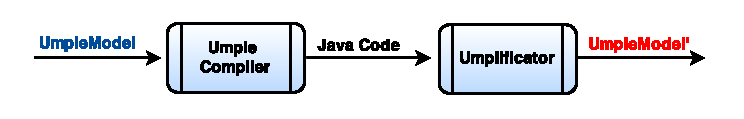
\includegraphics{Figures/preValidation.pdf} 
\caption{The Pre-Validation Phase: Comparing UmpleModel and UmpleModel'}
\label{fig:preValidation}
\end{figure}

Table \ref{table:umpleexamples} lists the Umple examples used in this pre-validation phase, well as  some statistics about them (number of lines of code of the Umple model, the number of lines of code of the corresponding Java system and the number of Java classes).

\begin{table}
\caption{Small examples used for first phase of validation}
\label{table:umpleexamples}
\begin{tabularx}{\textwidth}{l|SSX}
\toprule
\rowcolor[HTML]{BBDAFF}
\textbf{Name} & \textbf{\#LOC of Umple} & \textbf{\#LOC of Java} & \textbf{\# of Java Files} \\ \hline
2DShapes & 44 & 509 & 9\\ \hline
AccessControl & 67 & 1560 & 6\\ \hline
Accidents & 42 & 730 & 4\\ \hline
Accommodations & 102 & 2215 & 9\\ \hline
AfghanRainDesign & 132 & 2610 & 13\\ \hline
Airline & 51 & 1800 & 8\\ \hline
Banking System A & 87 & 2400 & 13\\ \hline
Banking System B & 74 & 1650 & 12\\ \hline
Canal System & 69 & 2222 & 14\\ \hline
Decisions & 148 & 4153 & 15\\ \hline
Card Games (Oh Hell and Whist) & 134 & 2051 & 8\\ \hline
Claim (Insurance) & 19 & 408 & 2\\ \hline
Community Association & 68 & 1591 & 9\\ \hline
Co-op Education System & 69 & 2420 & 10\\ \hline
DMM Overview & 59 & 1165 & 10\\ \hline
DMM Source Object Hierarchy & 91 & 1774 & 16\\ \hline
DMM Relationship Hierarchy & 135 & 1119 & 31\\ \hline
DMM CTF & 93 & 932 & 4\\ \hline
Election System & 83 & 2875 & 11\\ \hline
Elevator System A & 42 & 1307 & 4\\ \hline
Elevator System B & 56 & 1971 &11\\ \hline
Genealogy A & 29 & 670 & 2\\ \hline
Genealogy B & 32 & 945 & 2\\ \hline
Genealogy C & 36 & 1017 & 3\\ \hline
Geographical Information System & 52 & 1174 & 11\\ \hline
Hospital & 65 & 1923 & 9\\ \hline
Hotel & 47 & 1888 & 10\\ \hline
Insurance & 63 & 1417 & 10\\ \hline
Inventory Management & 44 & 1753 & 7\\ \hline
Library & 42 & 1595 & 10\\ \hline
Mail Order System- Client Order & 38 & 1895 & 8\\ \hline
Manufacturing Plant Controller & 84 & 3089 & 11\\ \hline
Pizza System & 67 & 1555 & 9 \\ \hline
Police System & 64 & 3186 & 10\\ \hline
Political Entities & 32 & 842 & 5\\ \hline
Real Estate & 79 & 2071 & 8\\ \hline
Routes and Locations & 127 & 2089 & 9\\ \hline
School & 18 & 397 & 9\\ \hline
TelephoneSystem & 38 & 1838 & 7\\ \hline
University System & 32 & 1206 & 4\\ \hline
Vending Machine & 97 & 1696 & 8\\ \hline
WarehouseSystem & 83 & 2831 & 12\\ \hline
\hline
\end{tabularx}
\end{table}

For instance, the \textit{`Access Control Example'}, representing a system for managing access to facilities, is comprised of 6 classes, 8 associations, and 10 attributes. The Umple model is presented in Listing \ref{lst:accessControlEx} together with corresponding visual representation, a UML class diagram generated using our online tool (Figure \ref{fig:accessControlExample}). The unit test comparing the input umple model and the umplified model is shown in Listing \ref{lst:acsExample}.

\begin{lstlisting}[style=umpleIn,caption=Umple Model for an Access Control System, label=lst:accessControlEx]
namespace access_control;

class FacilityType
{
  code;
  description { Menu, Record, Screen }
  key {code}
}

//Functional_Area
class FunctionalArea
{
  String code;
  0..1 parent -- * FunctionalArea child;
  description { Hr, Finance }
  key {code}  
}

//Facility_Functional_Area
association
{
  * FunctionalArea -- * Facility;
}

class Facility
{
  Integer id;
  lazy Time t; 
  * -> 0..1 FacilityType;
  Integer access_count;
  name;
  description;
  other_details;
  
  key {id}
}

class Role
{
  code;
  role_description { Dba, ProjectMgr }
  
  key {code}
}

class User
{
  Integer id;
  * -> 0..1 Role;
  first_name;
  last_name;
  password;
  other_details;
  key {id}
}

associationClass RoleFacilityAccessRight
{
  * Facility;
  * Role;
  CRUD_Value { R, RW }
}
\end{lstlisting}
%http://yuml.me/4aab4a38
\begin{figure}[h]
\centering
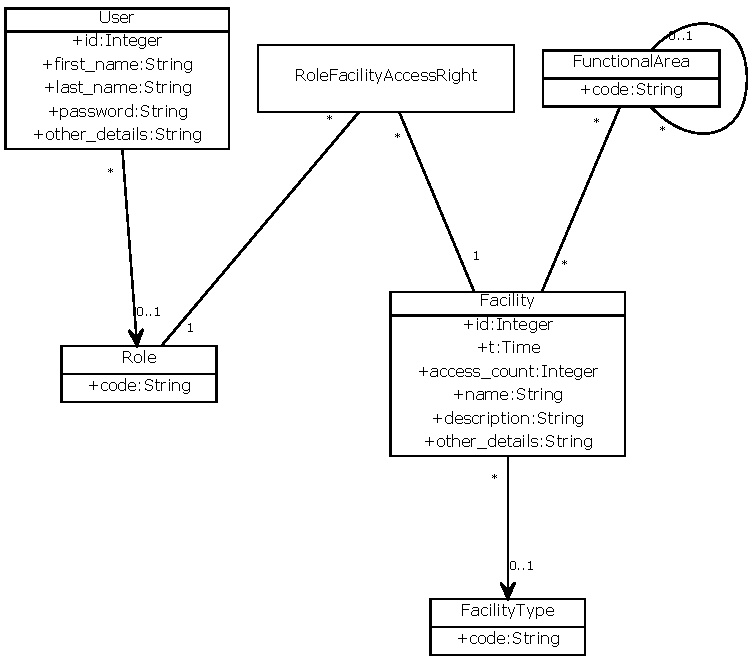
\includegraphics{Figures/accessControl.pdf} 
\caption{UML Class diagram of the Access Control system}
\label{fig:accessControlExample}
\end{figure}

\begin{lstlisting}[style=java,label={lst:acsExample},caption=Unit test to assert the Access Control Example.]
@Test
public void AccessControlExample(){
 String folderName = "AccessControl";
 File inputFile = new File(pathToRoot+ File.separator +folderName +".ump");
 UmpleFile inputUmpleFile = new UmpleFile(inputFile);
 // Umplify all the files in folder
 List<File> inputFiles = FileHelper.getListOfFilesFromPath(pathToRoot+ File.separator +       folderName, new ArrayList<File>());
 // Umplify files. Process must succeed!
 assertTrue(umplificator.umplify(inputFiles));
 // This is the actual model, the one umplified 
 UmpleModel umplifiedModel = umplificator.getOutputModel();
 UmpleModel expectedModel = new UmpleModel(inputUmpleFile);
 expectedModel.run();		
 //1. Class FacilityType
 UmpleClass facilityTypeA = umplifiedModel.getUmpleClass("FacilityType");
 UmpleClass facilityTypeE = expectedModel.getUmpleClass("FacilityType");		
 Assert.assertEquals(1, facilityTypeA.numberOfAttributes());
 Attribute lazyAttributeA = facilityTypeA.getAttribute("code");
 Attribute lazyAttributeE = facilityTypeE.getAttribute("code");	
 assertEquals(lazyAttributeA.getIsLazy(),lazyAttributeE.getIsLazy());
 assertEquals(lazyAttributeA.getType(),lazyAttributeE.getType());		
 // 2. Class User
 UmpleClass userA = umplifiedModel.getUmpleClass("User");
 UmpleClass userE = expectedModel.getUmpleClass("User");	
 Attribute id = userA.getAttribute("id");
 Attribute firstname = userA.getAttribute("first_name");
 Attribute lastname = userA.getAttribute("last_name");
 Attribute other_details = userA.getAttribute("other_details");
 Attribute password = userA.getAttribute("password");
		
 Assert.assertEquals(userA.numberOfAttributes(), userE.numberOfAttributes());
 Assert.assertEquals("Integer", id.getType());
 Assert.assertEquals("String", firstname.getType());
 Assert.assertEquals("String", lastname.getType());
 Assert.assertEquals("String", other_details.getType());
 Assert.assertEquals("String", password.getType());
 // 3. Facility Class
 UmpleClass facilityA = umplifiedModel.getUmpleClass("Facility");
 UmpleClass facilityE = expectedModel.getUmpleClass("Facility");
 Assert.assertEquals(facilityA.numberOfAttributes(), facilityE.numberOfAttributes());

 Attribute timeAttr = facilityA.getAttribute("t");
 Attribute idAttr = facilityA.getAttribute("id");
 Attribute accessAttr = facilityA.getAttribute("access_count");
 Attribute nameAttr = facilityA.getAttribute("name");
 Attribute descAttr = facilityA.getAttribute("description");
 Attribute otherAttr = facilityA.getAttribute("other_details");
		
 Assert.assertTrue(timeAttr.isIsLazy());
 Assert.assertFalse(idAttr.isIsLazy());
 Assert.assertFalse(accessAttr.isIsLazy());
 Assert.assertFalse(nameAttr.isIsLazy());
 Assert.assertFalse(descAttr.isIsLazy());
 Assert.assertFalse(otherAttr.isIsLazy());
 // Compare both models, generally
 assertTrue(areModelsEqual(umplifiedModel,expectedModel));
}
\end{lstlisting}

In the test case above, the level of refactoring includes only attributes (Umple associations have not been extracted) so we are interested in the classes, generalizations and the attributes of each class. We assert that the classes have been correctly detected and that the attributes in each class have been correctly extracted (attribute type, attribute name and additional features). For instance, in Line 49 we assert that the attributes is \textbf{lazy}, since the variable is not one of the parameters in the constructor of the Java class \textit{Facility} (Java code is not shown here).

% You mention line 69, but there are only 57 lines.
% MG. Fixed. Line 49.

This pre-validation essentially proves that the Umplificator works, at a basic level on a significant amount of Java code, but with a known and consistent structure. It was fairly easy to tailor our transformation rules to reverse-engineer code that we had generated ourselves. We know exactly what the structure of this code is; we know that it will be the same throughout each example, and we know that it will not change over time (or if it does change, at least we have control of both forward and reverse engineering). Pre-validation, says nothing about whether the Umplificator can work `in the wild', against unknown code. That is what we have to do in the next stages of validation.

Our pre-validation is similar to the concept of `dogfooding' \cite{ash2003web}, in that we are testing the Umplificator on our own code. But it is not `full' dogfooding since we have not yet attempted to convert the whole of the Umple compiler back from generated Java to Umple; the Umple compiler is very large and has a number of complexities that will make this a challenge we leave to future work.

% So I have deferred the mention of dogfooding to the last paragraph above, and have been 'honest' about it. It would be an interesting challenge to see if in fact the Umplificator could in fact reverse the generated compiler. If it could, that would be a huge thing.
% MG. Perfect. 


\section{Initial Phase of Validation}

Our next step was to apply the Umplificator to various open-source systems written in Java. We use freely available systems to facilitate comparisons and replications of our evaluation. We provide some information on these systems in Table \ref{table:umplifiedSystems} including their version, number of lines of code and the number of classes.

Furthermore, we perform `\textit{manual}' umplification on all open-source systems in \ref{table:umplifiedSystems}. The results of the manual umplification are then compared to the results of our '\textit{automated}' umplification. 

We call this phase the `Initial' phase of validation because this is the first phase where we show that the Umplificator can work on systems that we have not created ourselves.

\begin{table}
\caption{Open-source systems umplified}
\label{table:umplifiedSystems}
\begin{tabularx}{\textwidth}{l|YSSY}
\toprule
\rowcolor[HTML]{BBDAFF}
\textbf{Name} & \textbf{Version} & \textbf{LOC} & \textbf{\# of Classes} \\ \hline
 1. JHotDraw \cite{jhotdraw}                   & 7.5.1   & 82132   & 694      \\ 
\hline 2.  Weka \cite{wekasvn}      & 3.7.13  & 278642  & 1370        \\ 
\hline  3. Java Bug Reporting Tool\cite{jbrtsvn} 		& 1.0     & 2629    & 27        \\ 
\hline  4. JEdit\cite{jeditsvn}                   	& 1.12    & 59699   & 84         \\ 
\hline  5. FreeMaker\cite{freemakersvn}               & 2.3.15  & 39864   & 131         \\ 
\hline  6. Java Financial Library\cite{jflsvn}  		& 1.6.1   & 1248    & 28          \\ 
\hline  7. Args4j\cite{args4jsvn}                 	 & 2.0.30  & 2223    & 61            \\
\hline
\end{tabularx}
\end{table}

More concisely, for each system studied, we have followed these steps:

\begin{enumerate}
\item We apply the different transformation steps on the input object-oriented system.

\item We run the test suite available for the system to ensure that code compiles and is semantically identical to the original input source code.

\item We run a custom-made code analyzer on the Umple system generated (umplified) to obtain the statistics of the detected (extracted) Umple constructs (attributes, associations). At this stage, we obtain the number of attributes extracted for each class, their type, as well as the number of all different types of associations.	

\item We compare our results with data obtained from manual umplification. That is, we umplify the system without the help of the Umplificator tool. The manual 	umplification, a very time consuming task, is usually performed by another software engineer (undergraduate students contributing to the Umple project). 

\item We compute the \textit{precision} and \textit{recall} of the results previously obtained. Precision assesses the proportion of the constructs (attributes, associations) identified that are valid -- in other words that were also identified by the manual umplification. Recall assesses the proportion of the independently-identified constructs that are found by our approach (a number near 1 would means very few are missed by our detection algorithms). 

\item We refine our mapping rules to improve the precision of our algorithms. This step mainly concerns tuning the Umplificator. In general, tuning the Umplificator to increase its accuracy includes one or more of the following manual steps:

	\begin{enumerate}
		\item If there is an Umple construct that was missed from the extraction (false negative), we may add a new mapping rule to cover this case.
		
		\item If there is an Umple construct that was incorrectly identified (false positive), we may edit the corresponding mapping rule.
		\item If one of the methods requiring additional transformations (as described in Table \ref{table:transformations}) was incorrectly refactored, we may review and correct the refactoring action (a function in Drools language) that led to the incorrect piece of code.
% The above sentence does not have an ending; also it makes reference to a table that does not yet exist
% MG. Fixed.		
	\end{enumerate}
Briefly, the complexity of the tuning our tool depends on the number of false positives and false negatives that the tool generates. 
\end{enumerate}

The following are the definitions we have employed for the precision and recall measures \cite{precisionRecallDef}:

% You have massively messed up here in multiple ways. Going forward as an independent researcher, you need to be able to detect these sorts of error yourself; by proofreading.
% Firstly, in your version I have put in comments below you were saying 'The intersection of the True positives and the True positives;' in both numerators! The numerator is always 'True positives'. It turns out that the union of any set with itself is itself, but nonetheless the numberator is nonsense. You have this right later on when you give the example. I think the issue was quite simply one of how you structured the Latex after I asked you to make a change -- it was putting the second half of the denominator in the numerator. But the problem is you never looked closely at the equation as out put.
% Secondly Your denominators are totally wrong. See my correction.
% Thirdly, you have put the 'magnitude' symbols around the sets before applying the intersection operator, so you are taking the intersection of integers!

% Below is what you had
%\[  Precision=\frac{|TP| \cap  |TP|}{|FP|}\]
%and \\
%\[  Recall=\frac{|TP| \cap |TP|}{|FN|} \]

% Below I have corrected it
% MG. Thanks for the correction. I have the equations right in mind, but I didn't check the pdf output.

\[  Precision=\frac{|TP|}{|TP \cap FP|}\]
and \\
\[  Recall=\frac{|TP|}{|TP \cap FN|}\]

Where,
\begin{enumerate}
\label{sec:tuning}
\item \textbf{TP} is the number of true positives. They correspond to modeling construct that were correctly identified by our algorithms. 
\item \textbf{FN} is the number of false negatives.  In the context of this work, they correspond to constructs that were missed from the automated umplification. 
\item \textbf{FP} is the number of false positives. They correspond to modeling constructs that were misidentified (false alarms). 
\end{enumerate}

The next sub-section presents the results of this validation stage. Specifically, we will present the statistics on the number of umple constructs recovered from the various open-source projects in \ref{table:umplifiedSystems} as well as the \textit{precision} and \textit{recall} measures. It is important to recall at this point that the resulting output artifact from manual umplification and automated umplification is in both cases an Umple model. We run our code analyzer on the resulting umple model to get statistics and the information required for our comparisons. For instance, if we run the code analyzer on two(fictitious) models, one being the result of manual umplification (\textit{ManualModel}) and the other one the result of automated umplification (\textit{AutomatedModel}) of the same input system and we obtain the following results:

For \textit{ManualModel}:
\begin{enumerate}
\item ManualModel contains 1 class = \{A\}
\item Class A contains 3 attributes = \{a,b,c\}
\end{enumerate}

For \textit{AutomatedModel}:
\begin{enumerate}
\item AutomatedModel contains 1 class = \{A\}
\item Class A contains 3 attributes = \{a,b,d\}
\end{enumerate}

We can then compute the precision and recall measures. In our fictitious example above, the results are as follows:

\begin{enumerate}
\item True positives: 2 relevant attributes were correctly retrieved \{a,b\}
\item False negatives:  1 attribute was missed \{c\}
\item False positives: 1 attribute was incorrectly retrieved \{d\}
\end{enumerate}

The precision and recall for the recovery of attributes for our fictitious sample system is:

% You got the denominators backwards. I have fixed
% MG. Thanks for the correction.

\begin{enumerate}
\item \textbf{Precision}: TP / (TP + FP) = 2 / (2 + 1) = 66.7\%
\item \textbf{Recall}: TP / (TP + FN) =  2 / (2 + 1) = 66.7\%
\end{enumerate}

Finally, the code analyzer mentioned before is an Umple feature that can be run on the command line:

\vspace{\baselineskip}
\begin{lstlisting}[style=umplePlain]
   java -jar umple.jar -g CodeAnalysis Test.ump
\end{lstlisting}
or using our online tool as shown in Figure \ref{fig:onlineCodeAnalyzer}.

\begin{figure}[h]
\centering
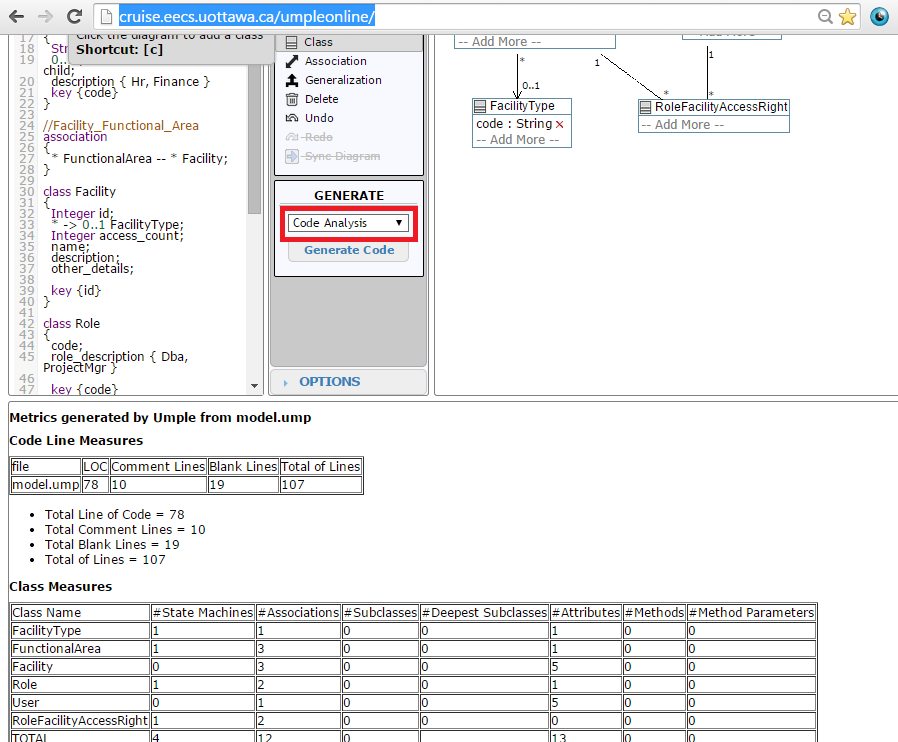
\includegraphics[width=0.75\textwidth]{Figures/UmpleOnlineCodeAnalyzer.png} 
\caption{Umple online - Code Analysis generation}
\label{fig:onlineCodeAnalyzer}
\end{figure}

\subsection{Results}

In the following tables we will present the number of initially recovered  attributes, and associations (of each type) for each of the systems studied. Nine different types of associations were identified in previous work \cite{UmpleAssociations}; we present results for three of them, corresponding to the top multiplicity patterns in industry: optional-one-to-many, optional-one-to-one and many-to-many associations.

The results below are a snapshot following the first attempt at automated umplification on these systems. That is, no tuning had been performed on the Umplificator to improve the results. Since then, after tuning the Umplificator,  the precision and recall measures for all open-source systems studied in Table \ref{table:umplifiedSystems} has been increased to 100\%.

Tables \ref{table:umplifiedResultsSystems1} - \ref{table:umplifiedResultsSystems7} detail the number of generalizations, the number of attributes and the different types of associations for the systems studied.

% Above you said 'remaining systems studied'. But the systems in these tables are the same systems as in the earlier umplifiedSystems tables. It took out the word 'remaining'.

% Above you say generalizations, but they do not appear in the tables.
% MG. I removed it. I didn't count them.
% Above the list of tables excludes JHotDraw. Not clear why.Below it includes jHotDraw,
% MG. Fixed. Mistake of my part.

% There is no table for Args4J. Any reason?
% MG. I added it. 

The second column of Tables \ref{table:umplifiedResultsSystems1} - \ref{table:umplifiedResultsSystems7} presents the number of Umple constructs that were correctly recovered (True positives). The third column presents the number of Umple constructs that were incorrectly recovered (False positives). The fourth column presents the number of expected Umple constructs (True Positives + False Negatives, resulting from manual umplification). The last two columns present the precision and recall computations. Note that the number of missed Umple constructs (False negatives) can be computed by subtracting the number of correctly retrieved Umple constructs from the number of expected Umple constructs. 
% Note that I again had to fix your math in the last sentence above. This is a clear weakness you will have to pay attention to.
% The headings of the last three columns in the tables is being cut off.
% MG Fixed.
Let us look specifically at one of the tables, Table \ref{table:umplifiedResultsSystems1}; this shows the results of detection of Umple constructs for the JHotDraw framework.  It shows that for JHotdraw, 383 of the attributes were recovered; however only 95\% were actual attributes. It turns out that, 20 1-to-1 associations were mistakenly extracted as attributes. More details concerning the Umplification of JHotdraw and Weka will be given in Section \ref{sec:6CaseStudies}.

\begin{table}[h]
\caption{Results of umplification for JHotDraw}
\label{table:umplifiedResultsSystems1}
\centering 
\begin{tabularx}{\textwidth}{l|ccccc}
\toprule
\rowcolor[HTML]{BBDAFF}
\textbf{} & \textbf{TP}  & \textbf{FP} & \textbf{Expected} & \textbf{Precision}  & \textbf{Recall}\\ \hline
Attributes & 383  & 20  & 363  & 95\% & 100\% \\ \hline
Associations optional-one-to-many &  22 & 0 & 49 & 100\% & 45\% \\
Associations optional-one-to-one &  115 & 0 & 185  & 100\% & 62.2\% \\ 
Associations many-to-many & 30 & 0 & 32 & 100\% & 93.8\%\\ 
\end{tabularx}
\end{table}

\begin{table}[h]
\caption{Results of umplification for Weka}
\label{table:umplifiedResultsSystems2}
\begin{tabularx}{\textwidth}{l|ccccc}
\toprule
\rowcolor[HTML]{BBDAFF}
\textbf{} & \textbf{TP}  & \textbf{FP}  & \textbf{Expected} & \textbf{Precision}  & \textbf{Recall}\\ \hline
Attributes & 1281	& 0	& 1510 & 100\%	& 84.9\% \\ \hline
Associations optional-one-to-many &  168 & 0 & 442 & 100\% & 38\% \\
Associations optional-one-to-one &  224 & 12 & 285 & 94.92\%  & 86.8\% \\ 
Associations many-to-many & 89 & 0 & 115 & 100\% & 77.4\% \\ 
\end{tabularx}
\end{table}

\begin{table}[h]
\caption{Results of umplification for the Java Bug Reporting Tool}
\label{table:umplifiedResultsSystems3}
\begin{tabularx}{\textwidth}{l|ccccc}
\toprule
\rowcolor[HTML]{BBDAFF}
\textbf{} & \textbf{TP}  & \textbf{FP}  & \textbf{Expected} & \textbf{Precision}  & \textbf{Recall}\\ \hline
Attributes & 31 & 0  & 31  & 100\% & 100\% \\ \hline
Associations optional-one-to-many &  9 & 0 & 12  & 100\%& 75\% \\
Associations optional-one-to-one &  4  & 0 & 4  & 100\% & 100\% \\ 
Associations many-to-many & 7 & 0 & 7 & 100\% & 100\%\\ 
\end{tabularx}
\end{table}

\begin{table}[h]
\caption{Results of umplification for JEdit}
\label{table:umplifiedResultsSystems4}
\begin{tabularx}{\textwidth}{l|ccccc}
\toprule
\rowcolor[HTML]{BBDAFF}
\textbf{} & \textbf{TP}  & \textbf{FP}  & \textbf{Expected} & \textbf{Precision}  & \textbf{Recall}\\ \hline
Attributes & 30  & 1 & 30 & 96.8\% & 100\%\\ \hline
Associations optional-one-to-many & 15  & 0 & 15  & 100\% & 100\% \\ 
Associations optional-one-to-one  &  22 & 0 & 22 & 100\% & 100\% \\
Associations many-to-many &  40 & 0 & 48  & 100\% & 83.3\% \\ 
\end{tabularx}
\end{table}

\begin{table}[h]
\caption{Results of umplification for FreeMaker}
\label{table:umplifiedResultsSystems5}
\begin{tabularx}{\textwidth}{l|ccccc}
\toprule
\rowcolor[HTML]{BBDAFF}
\textbf{} & \textbf{TP}  & \textbf{FP} & \textbf{Expected}  & \textbf{Precision}  & \textbf{Recall}\\ \hline
Attributes & 140  & 0  & 140  & 100\% & 100\% \\ \hline
Associations optional-one-to-many &  37 & 0 & 38 & 100\% & 97.4\% \\
Associations optional-one-to-one &  29 & 0 & 29  & 100\% & 100\% \\ 
Associations many-to-many & 50 & 0 & 52 & 100\% & 96.2\%\\ 
\end{tabularx}
\end{table}

\begin{table}[h]
\caption{Results of umplification for the Java Financial Library}
\label{table:umplifiedResultsSystems6}
\begin{tabularx}{\textwidth}{l|ccccc}
\toprule
\rowcolor[HTML]{BBDAFF}
\textbf{} & \textbf{TP}  & \textbf{FP} & \textbf{Expected}  & \textbf{Precision}  & \textbf{Recall}\\ \hline
Attributes & 15  & 0  & 15  & 100\% & 100\%  \\ \hline
Associations optional-one-to-many &  8 & 0 & 8 & 100\% & 100\%\\
Associations optional-one-to-one &  30 & 0 & 30  & 100\% & 100\% \\ 
Associations many-to-many & 12 & 0 & 12 & 100\% & 100\% \\ 
\end{tabularx}
\end{table}

\begin{table}[h]
\caption{Results of umplification for Args4j}
\label{table:umplifiedResultsSystems7}
\begin{tabularx}{\textwidth}{l|ccccc}
\toprule
\rowcolor[HTML]{BBDAFF}
\textbf{} & \textbf{TP}  & \textbf{FP} & \textbf{Expected}  & \textbf{Precision}  & \textbf{Recall}\\ \hline
Attributes & 186 & 5 & 186 & 97.4\% & 100\%  \\ \hline
Associations optional-one-to-many &  12 & 0 & 12 & 100\% & 100\%\\
Associations optional-one-to-one &  4 & 0 & 5  & 100\% & 100\% \\ 
Associations many-to-many & 28 & 0 & 28 & 100\% & 100\% \\ 
\end{tabularx}
\end{table}

By studying the tables, we can see that the recall rate of our detection algorithms (before tuning) was at its absolute minimum around 38\% but neared 100\% in many cases. Precision ranged between 95\% and 100\%.

An additional step we took was to instrument our forward and reverse engineering framework components with timers to measure the time taken to process an input Java file and produce the target source code. More specifically, the timer measures the time taken to 
\begin{enumerate*}
\item parse an input file,  \item build (extract) an instance of the base language model,   \item  transform the input model based on a predefined set of mapping rules into an Umple model, and \item generate code  (creating files with the .ump extension).
\end{enumerate*}

Table \ref{table:executionTimes} summarizes the execution times in milliseconds taken to reverse engineer two of the open-source systems in Table \ref{table:umplifiedSystems}. Note that the reverse engineering component uses Perf4J \cite{Perf4j} for calculating (and displaying) performance statistics. The values presented in Table \ref{table:executionTimes} correspond to the average of multiple execution times as gathered by this utility. Computation times do not include the time taken to compute metrics on the software systems. It is important to note that JHotdraw 

The tests were executed on a machine exhibiting the following characteristics:
\begin{itemize}
\item Intel Core i7-4500 CPU @ 3.10GHz  
\item RAM: 8.00 GB 
\item Windows 8 - 64 bits
\end{itemize}

\begin{table}[h]
\caption{Reverse engineering execution times}
\label{table:executionTimes} 
\begin{tabularx}{\textwidth}{X|SS}
\toprule
\rowcolor[HTML]{BBDAFF} 
  & \multicolumn{2}{l}{\textit{\textbf{Execution Time (in ms)}}} \\\hline
\textbf{Component}             & \textbf{JHotDraw}     & \textbf{Args4J}   \\\hline
\textbf{Parsing}               & 50899  & 12500         \\\hline
\textbf{Extractor}             & 21025  & 3204         \\\hline
\rowcolor{lightgray} 
\textbf{Transformer}           & 339327 & 920          \\\hline
\textbf{Generating Umple Code} & 1700   & 450          \\\hline
\textbf{Total Time:}           & 412951 & 14074        \\\hline
\end{tabularx}
\end{table}

% you could add a column showing the percentage that JHotDraw figures exceed Args4J. That will heelp people assess performance. There is an approximately 4000% difference in size.
% MG Added in the paragraph below.
It can be seen from the above that the transformer is the process that dominates the time, and performs substantially worse than linearly; the other processes perform better than linearly. The execution times for the Transformer process depend on the number of rules applied (based on the level of refactoring achieved) and on the size of input system (138 classes and 22 interfaces as for JHotDraw, for instance) and this explains the variations in the execution times from one system to another. Furthermore, for args4j where the code contains only a few instance variables that can become Umple constructs, the transformation stage has been performed very fast compared to the corresponding time for JHotdraw, a very rich system in terms of modeling abstractions. Note that JHotdraw possesses 81632 lines of code compared to args4j which is made of 2233 lines of code. The net result in the cases shown here is approximate linear scaling; however, given that the transformer takes so much time, it appears that for extremely large systems the time required may become extremely lengthy. On the other hand, umplification is expected to be a task that a project would only perform once per body of code, so extended transformation time might not actually pose a practical problem.

% Note how I have discussed the data in a little more depth
% MG. Noted. Thanks.
\section{Second Phase of Validation}

This phase of our validation approach will adapt the model often used in machine learning. We one set of systems as the `training set' and then take another set as the `testing set' to see how well the Umplificator performs on unknown systems.

Our initial training set is the set of systems we worked with in the previous phase.

We will adapt this process to be iterative; in other words, we  tune the system based on problems found when working with the testing set. One type of problem is  failure of the umplification to complete, at its various levels. Another type of problem is automatic umplification that doesn't match manual umplification of one of the test systems.

The testing set hence becomes a new `training set'. The idea is to pick yet another fresh testing set, and repeat. Over time the umplificator should get better and better.

To enable this form of validation, we developed a tool that randomly downloads open-source projects from repositories such as Google Code, GitHub and SourceForge.

The following are the first three steps of our process:

\begin{enumerate}
\item \textit{Download} 100 projects (randomly) from the mentioned repositories based on the following criteria: 
	\begin{enumerate}
	\item The system must be written in Java (we will extend this for C++ as part of future work)
	\item The system must be of medium-size or small-size. We determine this using the labels provided by the repository hosting service.
	\end{enumerate}
\item \textit{Umplify} the projects that have been downloaded into the file system. Attempt to umplify the project fully, and in case of any error, leave behind the result up to the last successful umplification level. For instance, if the Umplification failed at level 2 for one project, then stop the umplification for that project at level 1.

\item \textit{Report} the results following a similar directory structure as the downloaded project. The examples presented next will clarify this idea.
\end{enumerate}

Assuming that we download the projects in a directory called \textit{downloaded\_projects}. We then call the script with two positional arguments, the first is the path to the built umplificator, and the second is the path the to projects directory. That is:

\vspace{\baselineskip}
\begin{lstlisting}[style=umplePlain]
   umplifying_script.sh ~/umplificator.jar ~/downloaded_projects
\end{lstlisting}

The script, partially shown in Listing \ref{lst:script}, calls the umplificator.jar to umplify each of the projects at level 0 (Line 3), if it succeeds we continue to the next level and attempt level 1 (Line 12) and so on. 

\begin{lstlisting}[style=mine, label=lst:script, caption=Part of the script responsible to umplify and report results]
# Umplify all projects
for dir in "${to_umplify[@]}"; do
 java -jar $umplificator -level=0 -dir -path=$dir/umple_output $dir
 if [ $? -eq 0 ]; then 
 # if success: output 0-file and continue to next level
  touch $dir/0.umplify.score
 else 
 # if fail: output f-file and move to next project
  touch $dir/F.umplify.score
  continue
 fi
 java -jar $umplificator -level=1 -dir -path=$dir/umple_output $dir 
 if [ $? -eq 0 ]; then 
 # if success: output 0-file and continue to next level
  touch $dir/1.umplify.score
 else 
  # if fail: move to next project
  continue
fi
  # ... code omitted
done
\end{lstlisting}

The file system is employed to report the Umplification scores; we place a file containing logging information following the same directory structure as the input system being umplified. In other words, 
we generate a file with a name that follows this structure '\textit{umplify\_dir/project/version/myfile}':

Where \textit{myFile} will can be one the following:
\begin{itemize}
\item (Doesn't Exist) -- If the Umplificator hasn't even been run on that version yet
\item F.Umplify.Score.log -- If the Umplificator failed to even umplify the version to level 0
\item \{012\}.Umplify.Score.log -- If the Umplificator succeeds on a specific level, a file starting with that level number (a project can potentially have all 3 levels and therefore can have 3 of these files).
\end{itemize}

For instance, if we are running the script on JHotdraw 7.5.1, and we have successfully umplified it at level 2, then we will be able to find a file named \textit{2.Umplify.Score} as follows:

\vspace{\baselineskip}
\begin{lstlisting}[style=umplePlain]
   umplify_dir/org/jhotdraw/draw/7.5.1/2.Umplify.Score.log
\end{lstlisting}

% in the above you have .log at the end of the filename, but you don't mention that earlier
% MG. Fixed

These files will be used to log the time taken to umplify, the mapping rules activated for the umplification of that unit and/or any errors. Listing \ref{lst:loggingUmplificator} shows an example of the logging information that could be gathered in one of these files.
% MG. If listing is too big, I can reduce it.
\begin{lstlisting}[style=umplePlain, caption= Logging Information Sample gathered by the Umplificator, label=lst:loggingUmplificator]
12:30:37 DEBUG cruise.umplificator.UmplificatorMain - Configure Logger from log4j.properties
12:30:37 DEBUG cruise.umplificator.UmplificatorMain - Umplification process started!
12:30:37 DEBUG cruise.umplificator.core.Umplificator - start time : 1427733037483
12:30:37 INFO  cruise.umplificator.FileHelper - Files to be umplified: Student.java
12:30:37 DEBUG cruise.umplificator.rules.RuleRunner - Instantiate RuleRunner- 
12:30:37 DEBUG cruise.umplificator.rules.RuleService - RuleService.startRuleEngine
12:30:37 DEBUG cruise.umplificator.rules.RuleRunner - RuleRunner.addRuleFile - Add Rules to WM
12:30:39 DEBUG cruise.umplificator.rules.RuleRunner - RuleRunner.insertUmpleModel 
12:30:39 DEBUG cruise.umplificator.core.Umplificator - Input language is: .java
12:30:39 DEBUG cruise.umplificator.core.Umplificator - ---Input---
12:30:39 DEBUG cruise.umplificator.parser.JavaParser - Parsing Compilation Unit
12:30:40 DEBUG cruise.umplificator.parser.JavaParser - Initializing Java Visitor 
12:30:40 cruise.umplificator.visitor.JavaClassVisitor - Visiting TypeDeclarations-Student
12:30:40 DEBUG cruise.umplificator.visitor.JavaClassVisitor - Visiting FieldDeclarations-private int id;
12:30:40 DEBUG cruise.umplificator.visitor.JavaClassVisitor - Visiting MethodDeclarations-setId
12:30:40.DEBUG cruise.umplificator.rules.RuleRunner - RuleRunner.insertUmpleClass - Insert uClass into working memory
12:30:40 DEBUG cruise.umplificator.rules.RuleRunner - RuleRunner.fireAllRules -     Fire rules LEVEL2
12:30:40 INFO  cruise.umplificator.core.Umplificator - Umplification process completed!
12:30:40 DEBUG cruise.umplificator.FileHelper - --UmpleClass has been created for output\Student.ump--
12:30:40 DEBUG cruise.umplificator.core.Umplificator - Elapsed Time : 2643
12:30:40 DEBUG cruise.umplificator.core.Umplificator - Stop Time : start[1427733037483]
\end{lstlisting}

We then perform the following steps to complete this validation phase:

\begin{enumerate}[resume]
\item \textit{Fix} issues at level 0. We check the results for each of the umplified projects. We inspect the log file for each of the failed projects (F.umplify.score files) to determine what is root cause of the problem. We fix any issues and proceed with next step.

\item \textit{Fix} issues at levels 1 and 2. We check this time the projects that were not umplified at level 2. We fix any issues and proceed with the next step.

\item \textit{Collect} the statistics on the number of umplified constructs for all projects umplified.

\item \textit{Tune further} by manually umplifying a sample. We select one of the projects for manual umplification. The results of manual umplification are compared with those of the automated umplification using the \textit{CodeAnalyzer}. At this point, we tune the Umplificator (refer to beginning of section \ref{sec:tuning}) until there are no discrepancies between the two umplified versions. 

\item \textit{Re-umplify}. We attempt the umplification of the initial 100 projects again, and compare the statistical results with those of Step 3. Ideally, tuning the Umplificator to fix issues in steps 4, 5 and 7 has improved the effectiveness for other projects in the set.

\item \textit{Repeat}. We collect 100 more projects and apply steps 1-10. 
\end{enumerate}

For the 100 first projects used in this part of our study and after completion of steps 1 to 3, we obtained the following results:

\begin{itemize}
\item 100 Projects were successfully umplified at level 0. '\textit{Successfully}' means that the resulting umple code can generate valid Java code.

\item 68 Projects were successfully umplified at level 1. 

\item 55 Projects were successfully umplified at level 2.On-going work is being done to fix the issues (Step 5 above).
\end{itemize}

and the results below, after completion of steps 4 to 8:
\begin{itemize}
\item  From the 32 umplified projects that couldn't be umplified at level 1, 18 of these umplified projects when compiled generated uncompilable source code. The main problem resided in the usage of Generic Types. For instance, class \textit{BuiltInBinding} of open-source project \textit{Dagger} in Listing \ref{lst:genericType} declares a Generic Type and is umplified as shown in Listing \ref{lst:genericUmplified}. In fact, this Umple class will generate a Java class that will break all code related to instantiating class \textit{BuiltInBinding} (i.e., return new BuiltInBinding$<$Object$>$(...).
Since Umple does not supporting template parameters, we have employed the `top' construct as temporarily workaround (in Listing \ref{lst:genericUmplifiedTop}). Code inside the `top' construct is generated into a file corresponding to the name of the `top' construct. Generic classes in Umple will be considered future work.
\item After fixing issues related to Generic types. The 18 projects were correctly umplified at level 1.
\item The 14 remaining projects were successfully umplified after fixing issues related to misplaced code injections.
\item Rules for the detection of one-to-many associations were tuned resulting in an improvement of 4\% in the number of detected associations of this type (in average for the 100 projects).
\end{itemize}

\begin{lstlisting}[style=java, caption=BuiltInBinding.java, label=lst:genericType]
public class BuiltInBinding<T> {
  private String delegateKey;
  private final ClassLoader classLoader;
  private Binding<?> delegate;
  // The rest of the code is omitted
}
\end{lstlisting}

\begin{lstlisting}[style=umpleIn, caption=BuiltInBinding.ump (Invalid), label=lst:genericUmplified]
class BuiltInBinding {
  String delegateKey;
  private final ClassLoader classLoader;
  private Binding<?> delegate;
  // The rest of the code is omitted
}
\end{lstlisting}

\begin{lstlisting}[style=umpleIn, caption=BuiltInBinding.ump using the Top construct, label=lst:genericUmplifiedTop]
top BuiltInBinding {
 public class BuiltInBinding<T> {
   private String delegateKey;
   private final ClassLoader classLoader;
   private Binding<?> delegate;
   // The rest of the code is omitted
 }
}
\end{lstlisting}

The code for the script is published online and can be found in our code repository \cite{umpleRepository} in the following directory:

\url{cruise.umplificator/scripts/umplificator_all_projects.sh}.

The project surrounding the umplificator that automatically downloads, tracks and reports on various projects can be found at: 

\url{https://github.com/mgarzon/dlproj}.

% Will this umple-ucosp userid stick around -- is it totally under your control? Better to put in our main repo sooner rather than later.
% MG. I have forked it to my own repository. Once John is done with all modifications I can move it to the main umple repository or leave it there. I don't have permissions to fork into the umple rep (in github).

The umplified systems, statistical results and scoring reports are available online in our code repository \cite{umpleRepository} in the following directory:

\url{experiments/mgarzon/thesis/CH6Evaluation}.

% I have taken off svn/trunk since when we move to github it won't be in something called svn. Furthermore I don't like 'main_thesis'. Be more descriptive.
% MG. Fixed

% You say that the process involves repeating in the last step with 100 more projects. This is future work presumably.
% MG. Yes.
% You do need to report here how much better things are after tuning.

\section{Case Studies}
\label{sec:6CaseStudies}

We now discuss three case studies in more detail. We start by presenting our experiences with \textbf{JHotDraw} and \textbf{Weka}, the two larger systems we studied; then we present a third case study regarding \textbf{Args4j} in which we perform additional re-engineering tasks.

\subsection{JHotDraw}
 
JHotDraw7 \cite{jhotdraw} is an open source graphic editor that supports operations on many graphics file formats. It makes extensive use of software design patterns and has detailed documentation about its design. We selected JHotDraw for umplification to be able to apply our transformations on documented frameworks and to compare results with the documentation of these frameworks and the analyses performed by other tools \cite{jhotdraw}. For this research we worked with JHotDraw 7.5.1.

Table \ref{table:umplifiedResultsSystems1} showed the results of detection of Umple constructs for the JHotDraw framework during our first attempt. After improving and refining our rules, we have obtained a precision and recall of 100\%. Table \ref{table:problemsJHotDraw} summarizes some of problems encountered during the incremental transformation of JHotDraw. The last column indicates the type of change required to fix the problem and the component concerned by the change: \{Umple.Compiler, Umplificator.Parser, Umplificator.Transformer, Umplificator.Generator and/or Umple.Extractor\}. The refinements consisted of adding the Java idioms that our detection algorithms were not able to catch on the first attempt and tuning the Umple compiler to generate compilable code from some of the umplified classes.

\begin{table}[htbp]
\caption{Problems encountered while umplifying JHotDraw}
\label{table:problemsJHotDraw}
\centering
\begin{tabularx}{\textwidth}{X|X}
\toprule
\rowcolor[HTML]{BBDAFF}
\textbf{Problem Description}  & \textbf{Fix}  \\ \hline
\textbf{1.} The Umplificator correctly detected Abstract Classes but since Umple did not support abstract classes at the time. Java code generated from the umplified JHotDraw was having compilation issues.
  & Umple.Compiler: We added the ability to declare classes as abstract classes. Refer to issue 76 in our defect tracking list \cite{UmpleIssues}.  \\\hline
 
\textbf{2.} Annotations preceding variable declarations were correctly output by the Umplificator but not handled by the Umple compiler. That is, the Umple compiler was generating invalid code from classes having annotations preceding field declarations such as @NotNullable.
 & Umple.Compiler: Annotations and comments are now handled and appear at the right place in the generated code.  Refer to issue 427 in our defect tracking list \cite{UmpleIssues}\\ \hline

\textbf{3.} Attributes were not correctly recovered. 23 Attributes were declared as immutable when they were not. By analyzing the cases, we discovered that some fields had setters that were not following the standard conventions (i.e., setX()). For instance, in class \textit{ArrowTip}, the setter for field angle was named 'updateAngle' rather than setAngle(...).
  &  Umplificator.Transformer: The helper, in charge of analyzing method declarations to determine whether or not the method sets a given field, was updated to take into account this naming convention.\\ \hline
  
\textbf{4.} Independent enumerations (Enum X in file X.java) were correctly identified by the Umplificator; however the Umple compiler didn't handle them since it could at the time only generate classes and interfaces. 
  &  Umple.compiler: We introduced a new construct named 'top' to put extra code at the top level. Refer to issue 614 in our defect tracking list \cite{UmpleIssues} \\ \hline

\textbf{5.} \textit{package-info.java} files that are used to provide a home for package level documentation and package level annotations were not handle correctly.
  &  Umple.compiler: We employed the 'top' construct previously described.    
 \\ \hline
\end{tabularx}
\end{table}

The Umplificator (Generator component) can generate master files to regroup classes per package. The Master file includes other Umple files by means of the 'use' statement. This is shown in Figure \ref{fig:jhotdrawMasterDraw}. The file named 'Master\_org.jhotdraw.draw.ump' regroups all classes in package '\textit{org.jhotdraw.draw}' and is used to generate the UML class diagram presented in Figure  \ref{fig:jhotdrawUMLClass}.

\begin{figure}[h]
\centering
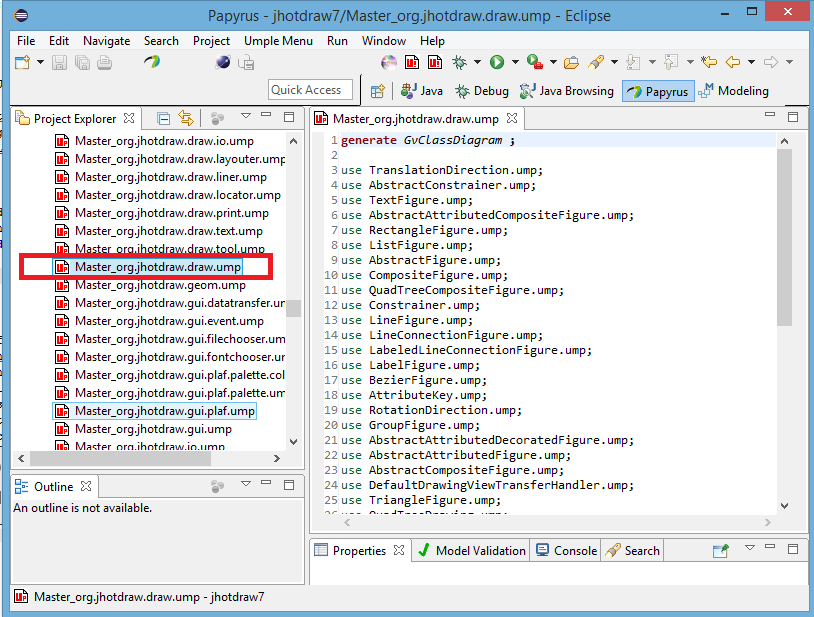
\includegraphics[width=0.80\textwidth]{Figures/jhotdrawMasterDraw.png} 
\caption{Master files used to compile JHotdraw}
\label{fig:jhotdrawMasterDraw}
\end{figure}

\newpage
\begin{sidewaysfigure}
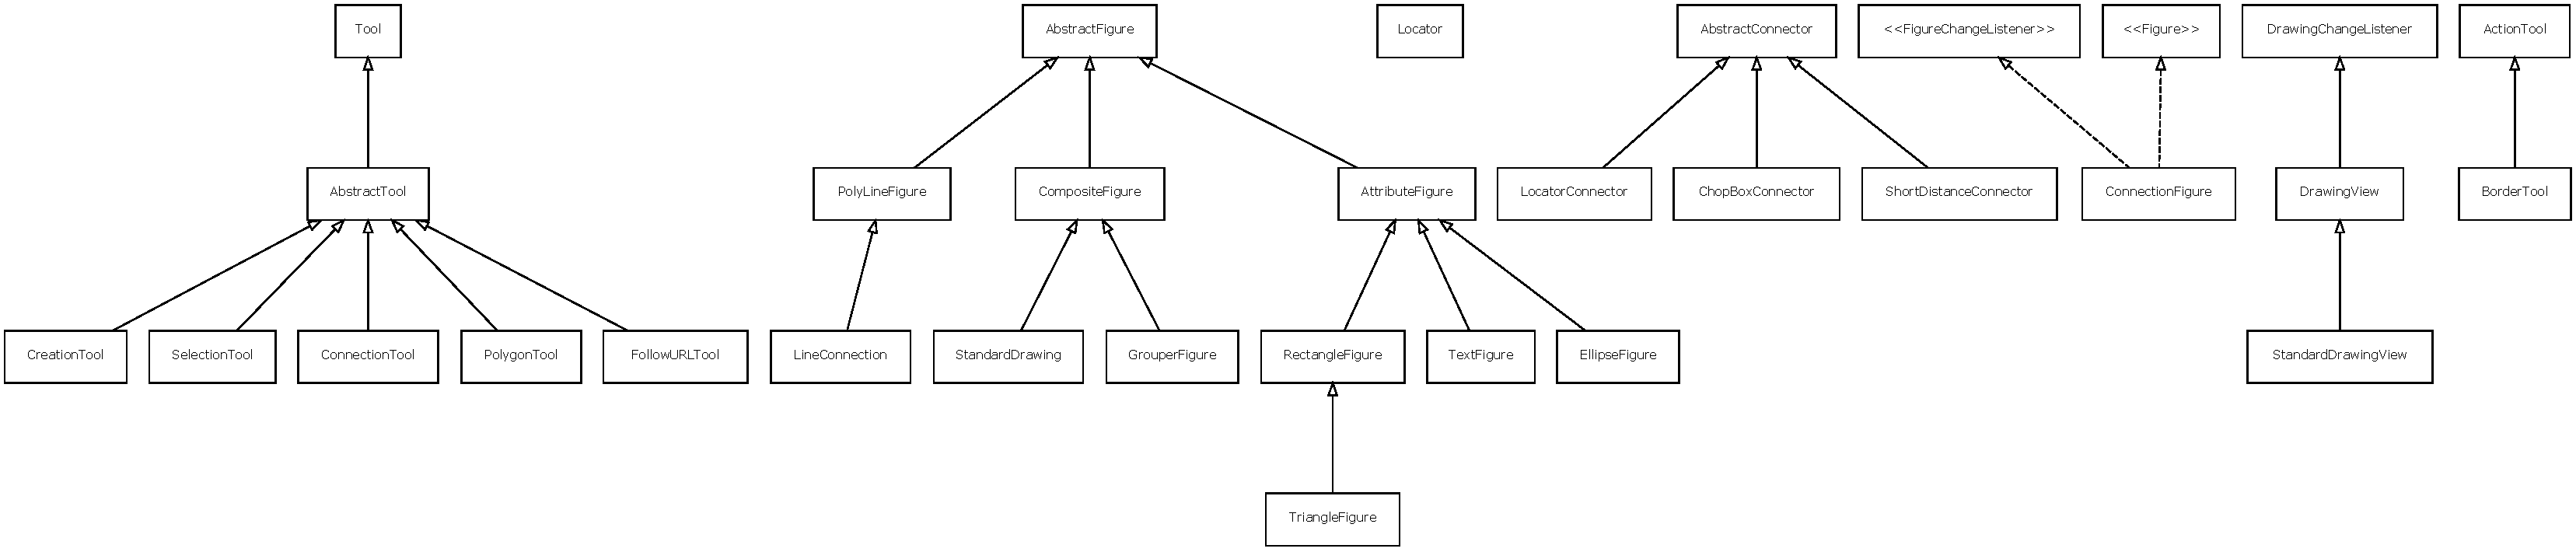
\includegraphics[width=0.99\textwidth]{Figures/jhotdrawuml.pdf} 
\caption{UML class diagram of package 'org.jhotdraw.draw' -  JHotdraw}
\label{fig:jhotdrawUMLClass}
\end{sidewaysfigure}

\subsection{Weka}
 
The next system we focused on was the machine learning tool Weka \cite{Weka}. As with our the first attempt at umplifying JHotDraw, our first attempt at automatically umplifying Weka resulted in the identification of the need for improvement to our rules; in particular some idioms it uses were not yet detected by our tool as it existed. For example, some classes in the classifiers package implement add() and remove() methods with different argument types. Also, the Confusion class declares add(RuleSet) and remove(Antecedent) to add and remove a set of rules from the evaluation algorithm. In addition, we detected, after execution of the test suite, that two classes were not compiling due to an unexpected constructor signature.

Another problem encountered while umplifying the Weka classes was related to inner classes. Classes such as \textit{weka.attributeSelection.BestFirst} that uses two inner classes to manage the nodes and linked lists in a best-first search. The Umplificator was attempting to match types inside other data types, resulting in an infinite loop. In addition, since the Umple compiler does not currently support inner classes, the solution chosen to remedy this situation was to ignore inner classes and processed them as Umple's `extra code'. 

Initial Umplification results for Weka nonetheless had a precision of 85\% when it comes to attributes and 38\% for 1-to-many associations. Table \ref{table:umplifiedResultsSystems1} summarizes the results. Note that a precision of 38\% doesn't mean that the Umplificator has missed 62\% associations of this type. It means that some of them were not correctly transformed into Umple (e.g. incorrect navigability, role names or transformation of accessor/mutator methods). The extensibility and flexibility of our tool allows us to add and refine rules without having to recompile the system. That is, rules in a external rule file (extension .drl) can be added to the working memory when running the Umplificator on the command line.

\subsection{Args4j - Modernization of the Code Base}

We reverse engineered Args4j \cite{UmpleFrameworkSANER15p494}, a small library that enhances the parsing of command line options and arguments in any Java application.

For every class in Args4j, our reverse engineering tool has produced two different files. The model design is expressed as an Umple model (i.e. Model.ump) and any algorithmic code is separated from the model (i.e. Model\_code.ump). Developers can now use the code generation technology to generate their system in any chosen programming language from the list of available languages in Umple.

If the modeler chooses to reproduce their system in the same language as it was before the reverse engineering process, we anticipate that the generated code will be of higher quality for a couple of reasons: First, we follow a rigorous test driven development approach in all of our framework components to ensure quality. Second, we have a state-of-the art code generator that respects associations multiplicity constraints and referential integrity \cite{UmpleAssociations}, and supports complex state machine code generation \cite{Badreddin2014EnhancedComposites}. Further details on the Umple API generated from various Umple constructs can be found at \cite{UmpleAPI}.

In another scenario, if the modeler chooses another programming language, as a target language, to generate the system, then they need to manually convert the algorithmic code in (files of type Model\_code.ump) to a new programming language such as C++. The distribution in terms of lines of code is as follows:

\begin{itemize}
\item Original Args4j Java source code is composed of 61 classes and 2223 lines of code.
\item Umplified Args4j source code is composed of 122 (2 per input class) umple files and 1980 lines of code in total.
\item Total number of lines of code in files containing modeling constructs (X.ump) is 312 LOC.
\item Total number lines of code in files with algorithmic/logic code (X\_code.ump) is 1668 LOC. If we exclude the umple class declarations and curly brackets, the number becomes 1424 LOC.
\end{itemize}

Consequently, to achieve the goal of translating Args4j into C++, a developer must translate 1518 lines of code (rather than 2223 lines of code). The benefits of umplification for the purposes of re-engineering may be more significant when processing larger software systems. This is marked as future work.

% Remind the reader here how much code would have to be rewritten with Umple being employed (algorithmic LOC number), vs the amount that would have to be rewritten (original LOC number) if Umple was not employed.
% MG. Done. Not great numbers however...
\section{Summary}

In this chapter, we have presented evaluation results showing that our approach and its current implementation are effective and efficient enough to be applied to real systems.
We have presented a multi-stage validation process evaluating the Umplificator from various perspectives.
and ensuring the quality of the transformations as well as the systems umplified by our tool. In the testing phase, we have presented an approach that independently tests the components of our tool. This is a generic approach that could be applied for the testing of programming languages, transformations technologies or compilers. In the pre-validation phase, we have tested the umplification process using our own set of examples while in the initial phase of validation we have used 7 commercial open source systems. The results show that by the precision and efficiency of the tool improves when more and more systems are umplified. Finally, the second validation phase, validates the Umplificator with a set 100 randomly selected projects. At this point of time, seven open-source and commercial projects have been fully reverse-engineered successfully and 100 randomly selected were successfully umplified at level 1 (attributes ). 

It is our continuous objective to successively umplify more and more systems, with the hope that eventually our rule base will cover the vast majority of cases needed to successfully umplify new systems the Umplificator is presented with. However, even with a precision in the high 80\% range, our tool serves as a useful tool for umplification. Users can leave some variables un-umplified, or can manually umplify the rest.  
% This leaves the reader hanging a little. At least recap the success rate for the 100 projects.
% MG. Added a bit more.